\section*{Research Context and Correlative Trends}

To ground the development of the \textbf{THERAPY} system in real-world public health trends, we conducted an exploratory data analysis using national datasets on suicide rates, drug overdose deaths, and mental health service access across the United States.

\subsection*{Background}

Suicide and overdose deaths have risen sharply in the U.S. over the past decade, prompting national concern and funding initiatives. While these outcomes are often discussed separately, we aimed to explore whether limitations in mental health infrastructure correlate with worsening public health trends.

We sourced data from the following publicly available datasets:

\begin{itemize}
  \item \textbf{CDC WONDER and Pressroom}: Suicide rates by state for 2022\autocite{cdc_suicide_2022}
  \item \textbf{CDC NVSS VSRR}: Provisional overdose death rates by state\autocite{cdc_overdose_2022}
  \item \textbf{SAMHSA NSUMHSS}: Percent of facilities in each state offering mental health treatment\autocite{samhsa_nsumhss_2023}
  \item \textbf{Kaggle WHO Dataset}: Historical suicide trends (1985–2016)\autocite{kaggle_suicide_1985_2016}
\end{itemize}

\subsection*{Analysis and Visualization}

We merged these datasets by state and performed basic correlative and nonlinear trend analysis to explore the hypothesis that access to care is inversely related to suicide and overdose rates.

\begin{figure}[H]
  \centering
  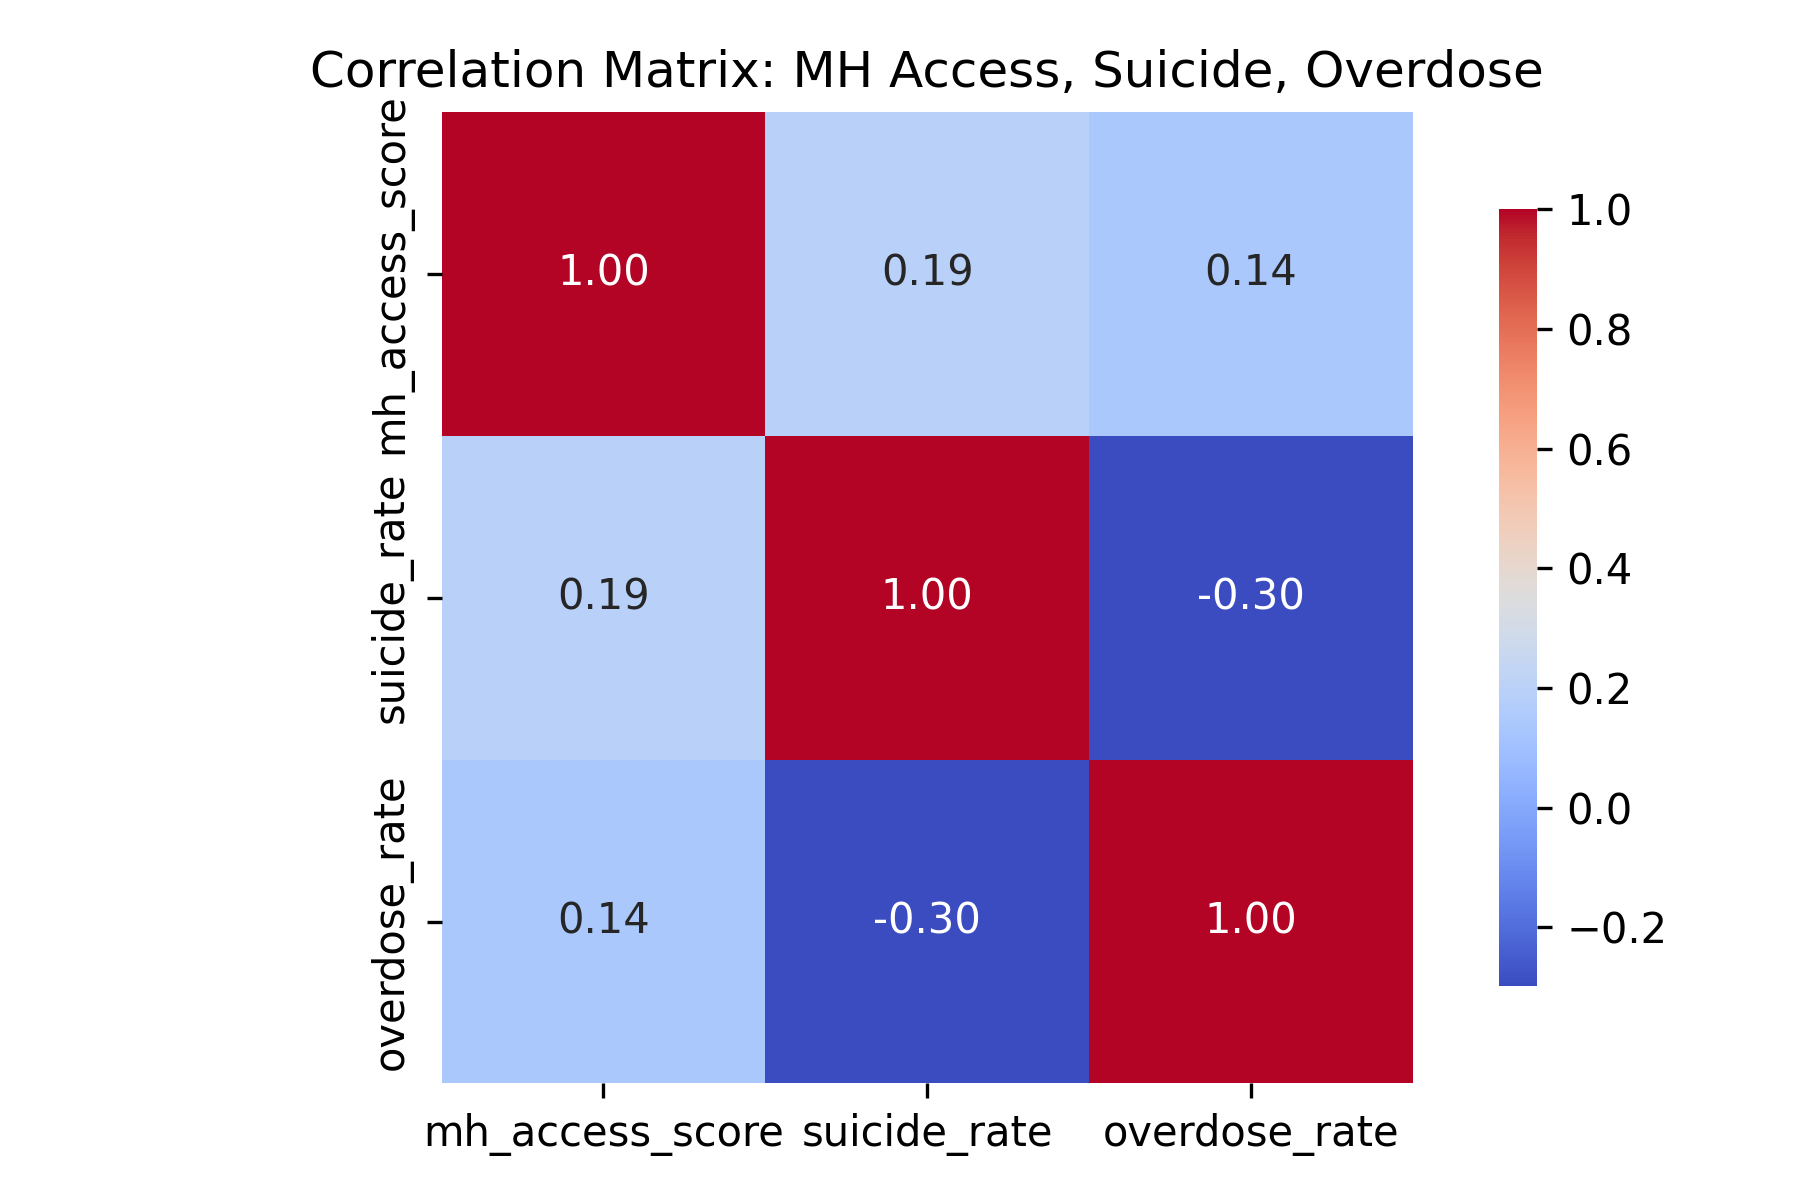
\includegraphics[width=0.85\textwidth]{correlation_matrix.png}
  \caption{Pearson correlation matrix of MH access, suicide rate, and overdose rate}
\end{figure}

\begin{figure}[H]
  \centering
  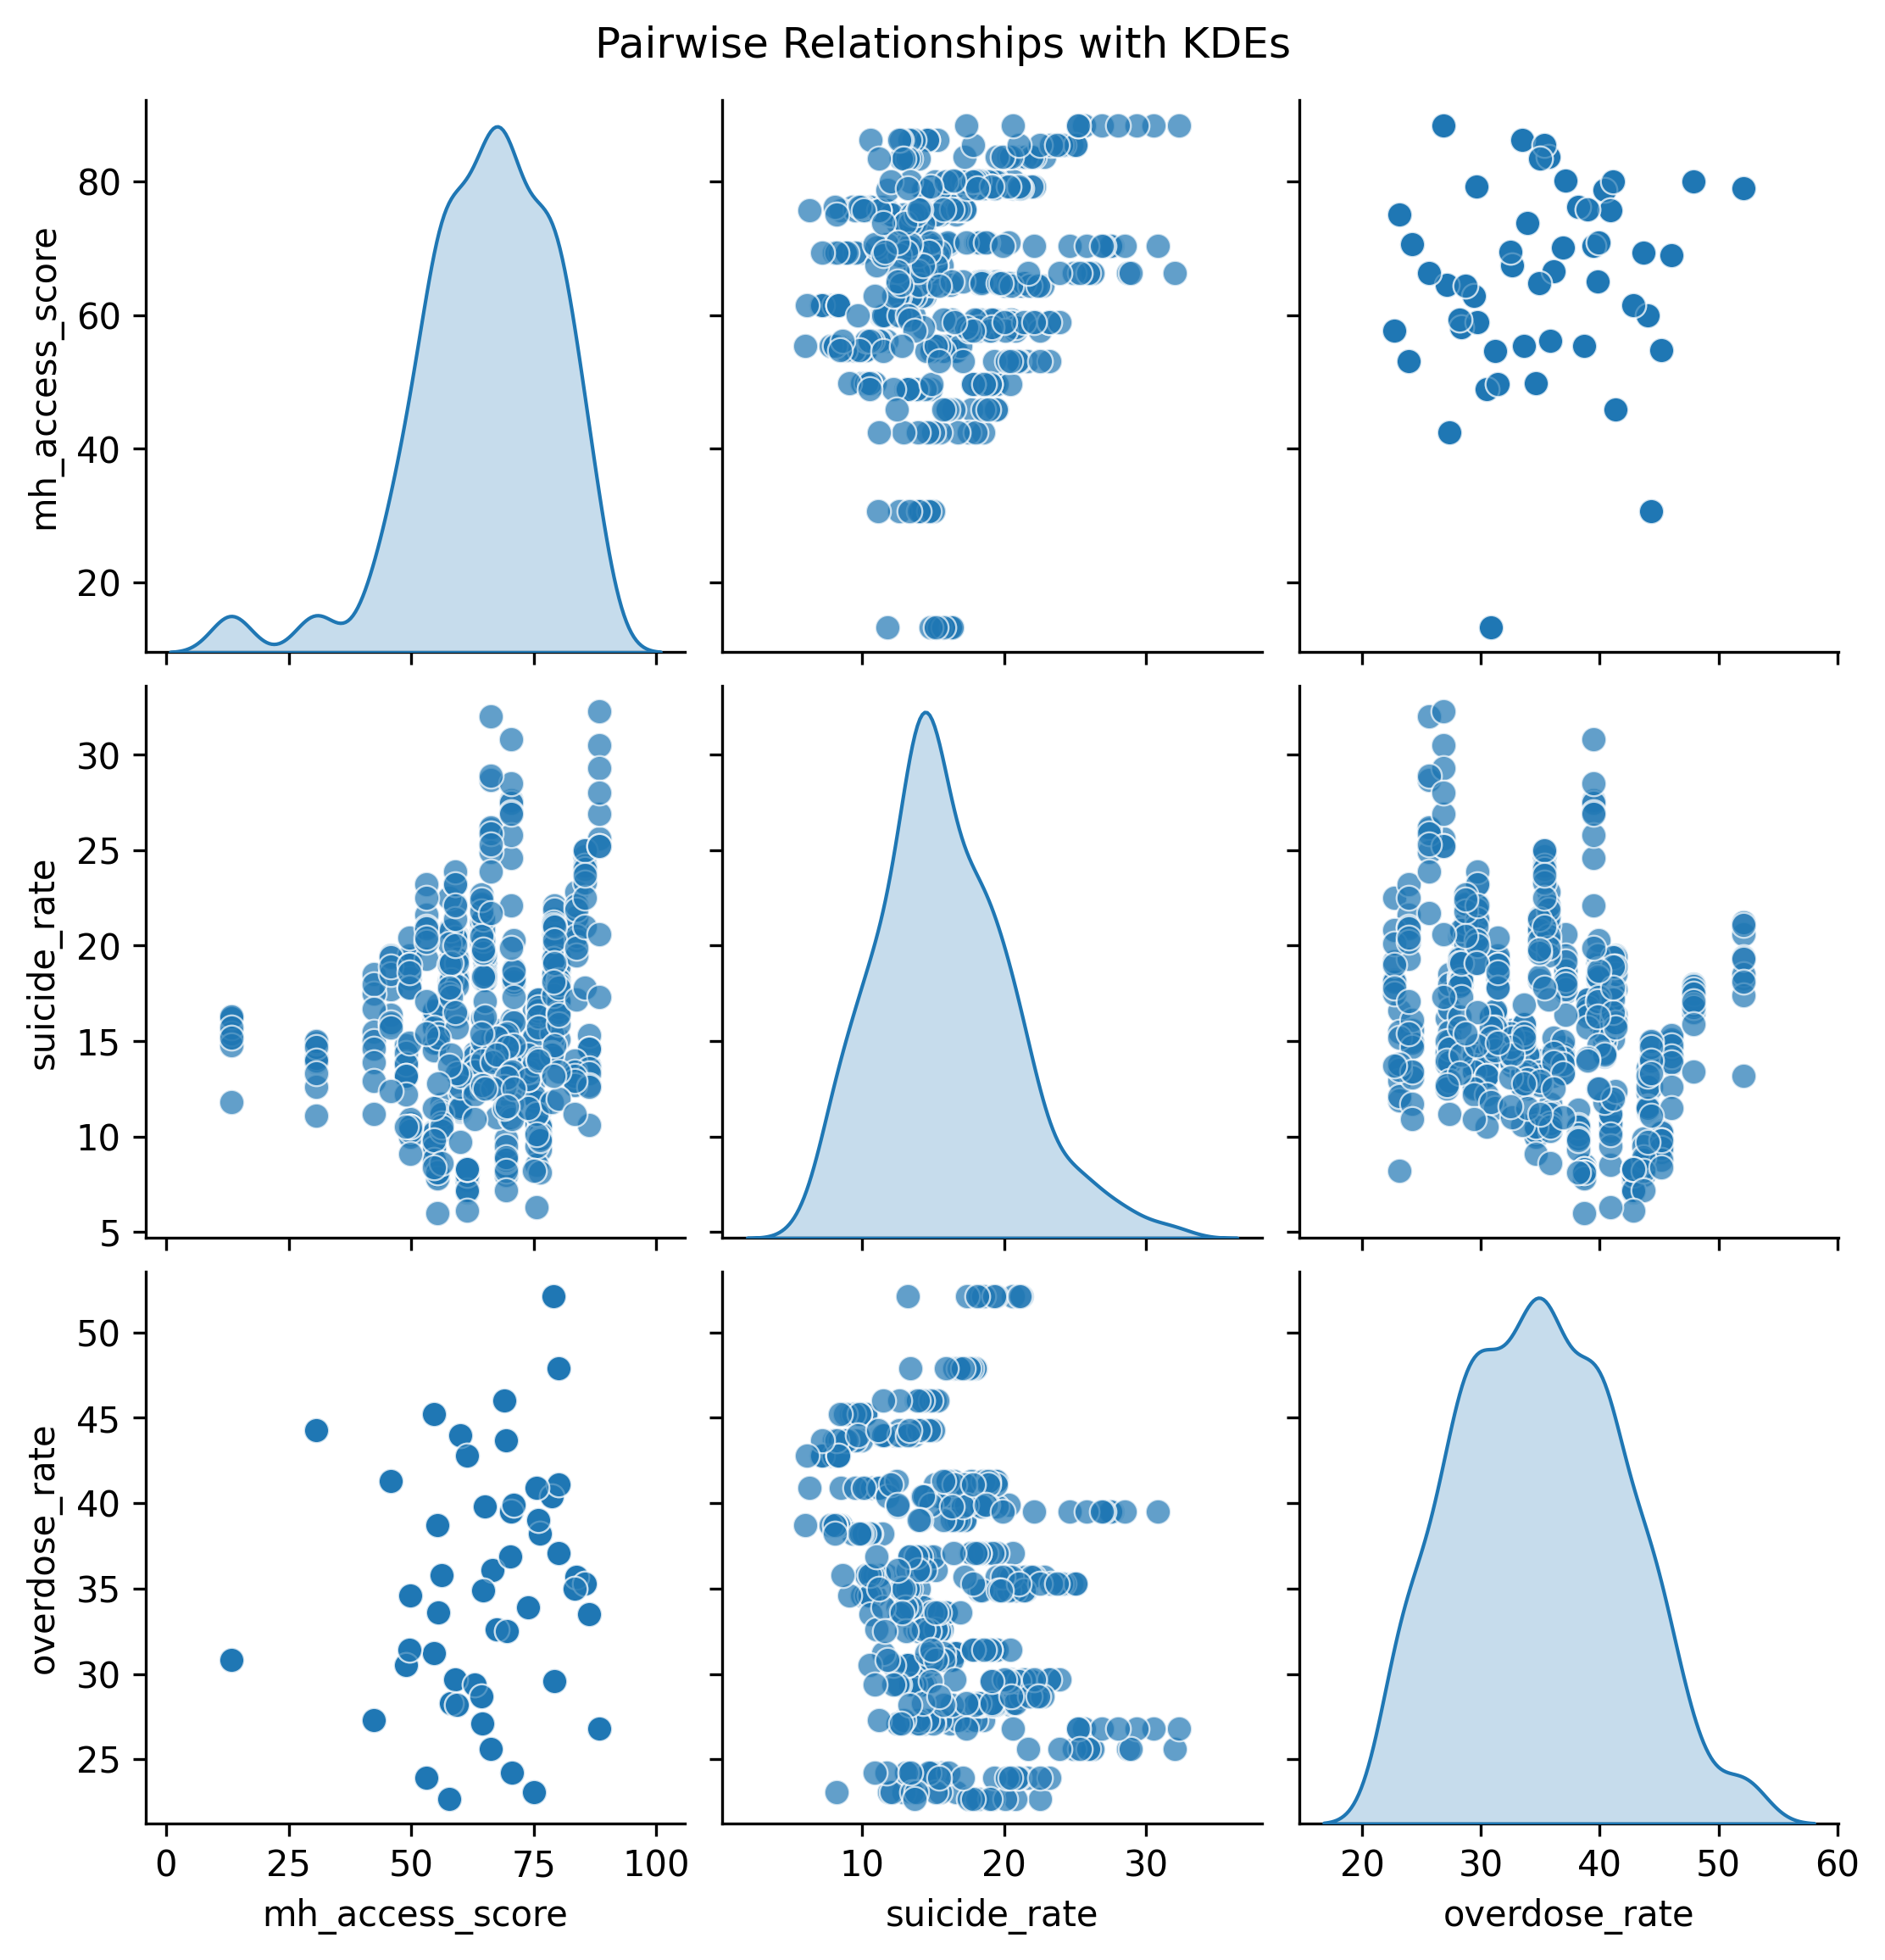
\includegraphics[width=0.85\textwidth]{pairwise_kde_plot.png}
  \caption{Pairwise relationships with kernel density estimates (KDEs)}
\end{figure}

\begin{figure}[H]
  \centering
  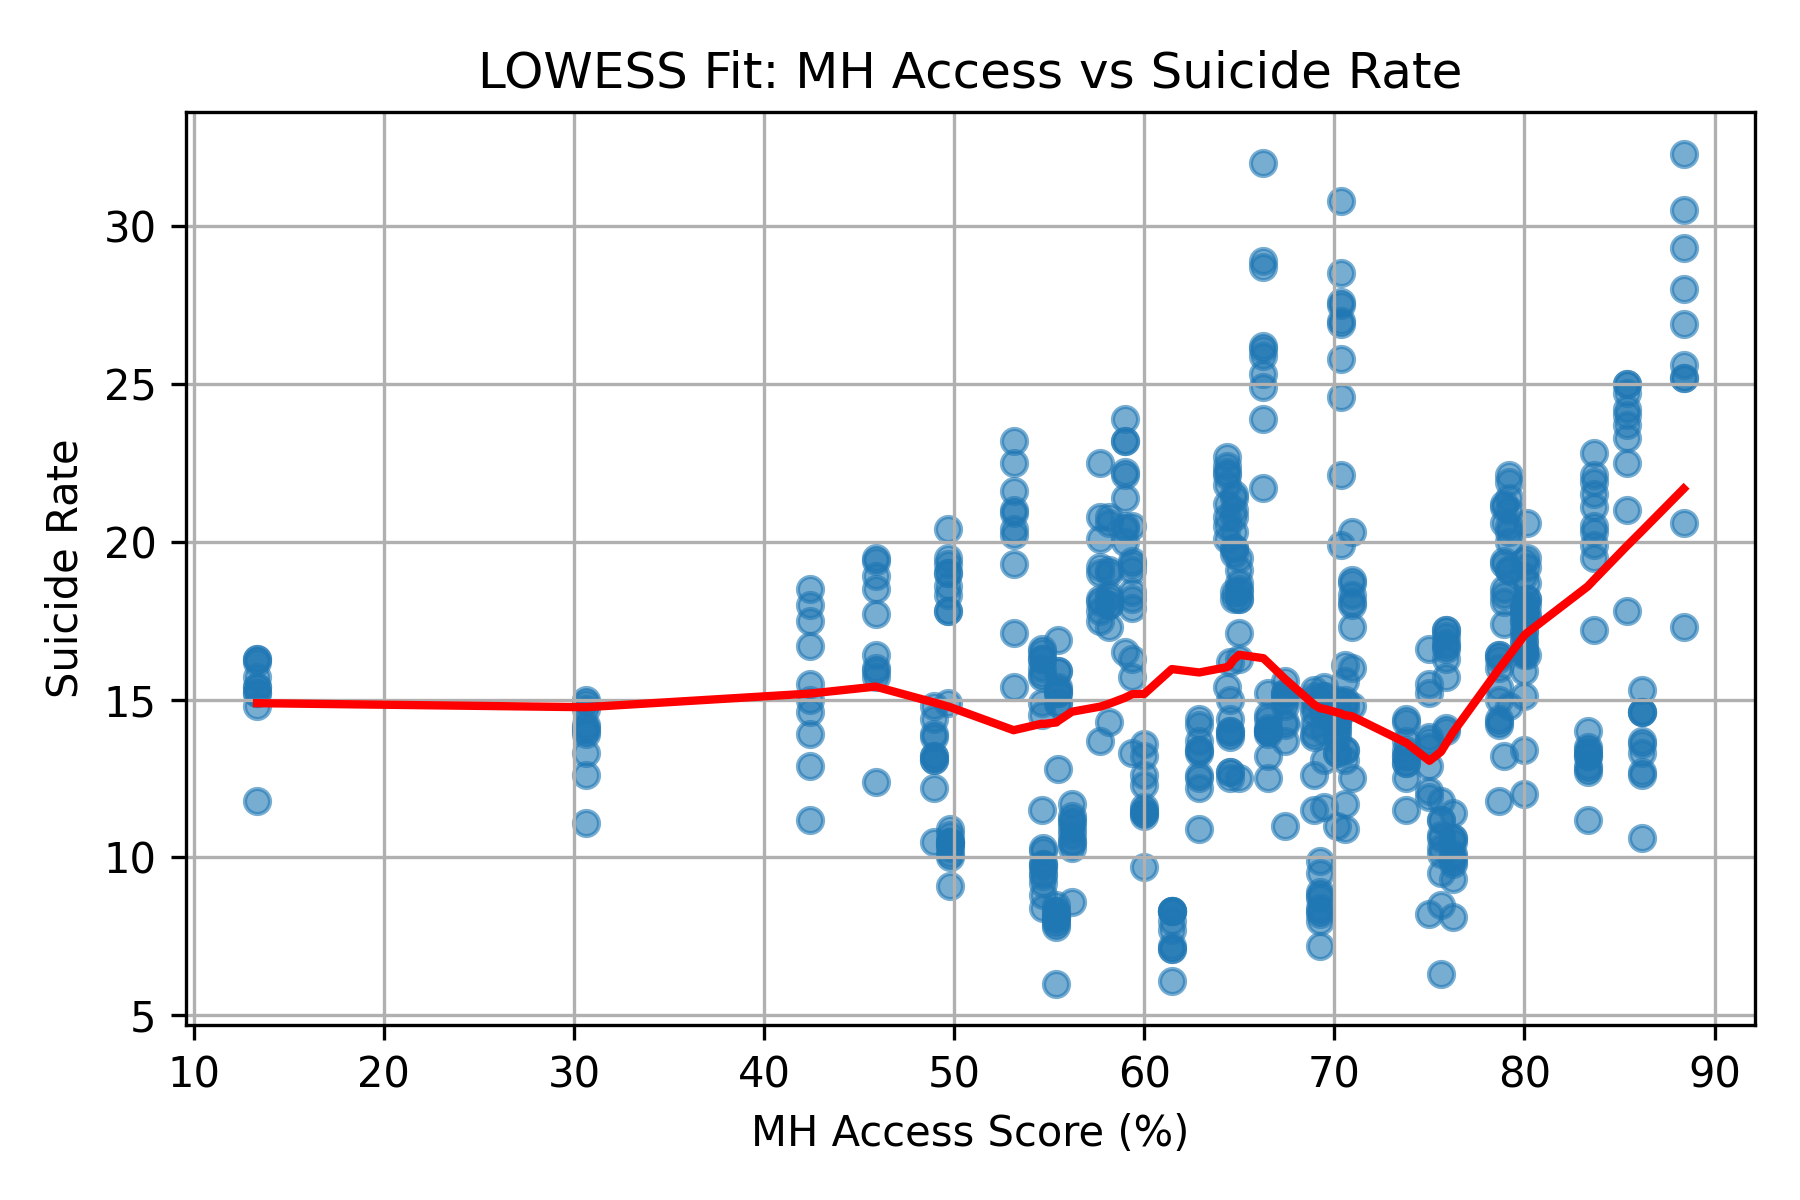
\includegraphics[width=0.85\textwidth]{lowess_suicide_vs_access.png}
  \caption{Nonlinear LOWESS fit of mental health access vs suicide rate}
\end{figure}

\subsection*{Interpretation}

Our analysis did not identify strong linear correlations between mental health access and suicide or overdose rates. However, nonlinear patterns suggest that the relationship may be more complex and context-dependent—possibly impacted by regional confounders, service delivery models, or lagging infrastructure response to emergent crises.

\subsection*{Implication}

This was not a conclusive statistical study, but a systems-level exploration. We believe this preliminary work highlights the potential value of an AI-assisted support layer—like \textbf{THERAPY}—to serve as a connective, privacy-respecting, and client-empowering layer of support between traditional care touchpoints. Future work may refine this analysis with longitudinal, demographic, and geospatial dimensions.

